\documentclass[8pt]{beamer}

\usetheme{Darmstadt}
\usecolortheme{orchid}
\usepackage[small,center]{caption}
\usepackage{times}
\usefonttheme{structurebold}
\usepackage[english]{babel}
\usepackage{pgf,pgfarrows,pgfnodes,pgfautomata,pgfheaps}
\usepackage{amsmath,amssymb,amsthm}

\usepackage{caption}
\usepackage{tikz}
\usetikzlibrary{shapes.misc}

\newcommand*{\vcenterimage}[1]{\vcenter{\hbox{\includegraphics[width=2in]{#1}}}}
\newcommand*{\vcenterarrow}{\vcenter{\hbox{$\Longrightarrow$}}}

\DeclareMathOperator{\hyphen}{-}

% \definecolor{RPIred}{rgb}{ 0.87,0.12, 0.20}
\definecolor{ballblue}{rgb}{0.13, 0.67, 0.8}
\definecolor{lightgray}{rgb}{0.83, 0.83, 0.83}
%\setbeamercolor{block title}{bg=lightgray,fg=RPIred}
\setbeamercolor{block body}{bg=white,fg=black}
\setbeamercovered{dynamic}
%\setbeamercolor*{item}{fg=RPIred}

\DeclareMathOperator*{\argmin}{arg\,min}

\captionsetup[subfigure]{labelformat=empty}
\captionsetup[figure]{labelformat=empty}
\setbeamertemplate{navigation symbols}{}
\setbeamertemplate{footline}[frame number]
\begin{document}

\newcommand{\matl}{M{\scriptsize ATLAB }}
\newcommand{\Div}[1]{\nabla\cdot #1}
\newcommand{\DIV}[1]{\nabla_{\mathbf{X}} \cdot #1}

\newcommand{\etal}{\emph{et al}.}

\newcommand{\BB}{\mathbb{B}}
\newcommand{\CC}{\mathbb{C}}
\newcommand{\FF}{\mathbb{F}}
\newcommand{\EE}{\mathbb{E}}
\newcommand{\PP}{\mathbb{P}}
\newcommand{\MM}{\mathbb{M}}
\newcommand{\FFb}{\overline{\FF}}

\newcommand{\ub}{\boldsymbol{u}}
\newcommand{\ubf}{\boldsymbol{u}^{\text{f}}}
\newcommand{\ubs}{\boldsymbol{u}^{\text{s}}}
\newcommand{\vb}{\boldsymbol{v}}
\newcommand{\wb}{\boldsymbol{w}}
\newcommand{\yb}{\boldsymbol{y}}
\newcommand{\Chib}{\boldsymbol{\chi}}
\newcommand{\cb}{\boldsymbol{\chi}}
\newcommand{\xb}{\boldsymbol{x}}
\newcommand{\Xb}{\boldsymbol{X}}
\newcommand{\fb}{\boldsymbol{f}}
\newcommand{\Fb}{\boldsymbol{F}}
\newcommand{\Tb}{\boldsymbol{T}}
\newcommand{\Ub}{\boldsymbol{U}}
\newcommand{\UbVecIB}{\vec{\Ub}\vphantom{\Ub}^{\text{IB}}}
\newcommand{\Vb}{\boldsymbol{V}}
\newcommand{\Lb}{\boldsymbol{L}}
\newcommand{\LbVecIB}{\vec{\Lb}\vphantom{\Lb}^{\text{IB}}}
\newcommand{\Nb}{\boldsymbol{N}}
\newcommand{\nb}{\boldsymbol{n}}
\newcommand{\hb}{\boldsymbol{h}}
\newcommand{\ab}{\boldsymbol{a}}
\newcommand{\Ab}{\boldsymbol{A}}
\newcommand{\phib}{\boldsymbol{\phi}}
\newcommand{\psib}{\boldsymbol{\psi}}

\newcommand{\cauchy}{\bbsigma}
\newcommand{\cauchyf}{\bbsigma^{\text{f}}}
\newcommand{\cauchyv}{\bbsigma^{\text{v}}}
\newcommand{\cauchys}{\bbsigma^{\text{e}}}
\newcommand{\cauchysolid}{\bbsigma^{\text{s}}}
\newcommand{\ztensor}{\mathbb{0}}
\newcommand{\pstab}{\pi_{\text{stab}}}
\newcommand{\pf}{\pi^{\text{f}}}
\newcommand{\ps}{\pi^{\text{s}}}
\newcommand{\pphys}{p}
\newcommand{\mus}{\mu^{\text{s}}}
\newcommand{\muf}{\mu^{\text{f}}}
\newcommand{\rhos}{\rho^{\text{s}}}
\newcommand{\rhof}{\rho^{\text{f}}}
\newcommand{\cbs}{\Chib^{\text{s}}}
\newcommand{\ds}{\boldsymbol{d}^{\text{s}}}

\newcommand{\PPs}{\PP^{\text{e}}}
\newcommand{\PPsm}{\bar{\PP}^{\text{e}}}

\newcommand{\soliddom}{{\Omega^{\text{s}}_t}}
\newcommand{\soliddomO}{{\Omega^{\text{s}}_0}}
\newcommand{\fluiddom}{\Omega^{\text{f}}_t}
\newcommand{\fluiddomO}{\Omega^{\text{f}}_0}
\newcommand{\fsinterface}{\Gamma^{\text{fs}}_t}
\newcommand{\fsinterfaceO}{\Gamma^{\text{fs}}_0}
\newcommand{\subsolid}{\omega^{\text{s}}_t}
\newcommand{\subsolidO}{\omega^{\text{s}}_0}

\newcommand{\Wiso}{W^{\text{iso}}}
\newcommand{\Wb}{\overline{W}}

\newcommand{\PPb}{\bar{\PP}^\text{e}}

\newcommand{\cNHB}{\bar{\cauchy}_{\text{NH}}}
\newcommand{\dev}{\text{dev}}
\newcommand{\DEV}{\text{DEV}}
\newcommand{\efac}{E_\text{FAC}}
\newcommand{\mfac}{M_\text{FAC}}
\newcommand{\tr}{\text{tr}}
\newcommand{\nus}{\nu_\text{stab}}
\newcommand{\kappas}{\kappa_\text{stab}}
\newcommand{\mul}{\mu_\text{L}}
\newcommand{\Gt}{G_\text{T}}
\newcommand{\Gl}{G_\text{L}}
\newcommand{\El}{E_\text{L}}

\newcommand{\vol}{\text{vol}}
\newcommand{\nvol}{\mathcal{N}}
\newcommand{\supp}{\text{supp}}
\newcommand{\mm}{\mathcal{M}}
\newcommand{\mmd}{\mathcal{M}^{\text{1D}}}
\newcommand{\xib}{\boldsymbol{\xi}}
\newcommand{\Pone}{\mathcal{P}^1}
\newcommand{\Ptwo}{\mathcal{P}^2}
\newcommand{\Qone}{\mathcal{Q}^1}
\newcommand{\Qtwo}{\mathcal{Q}^2}
\newcommand{\Bb}{\boldsymbol{B}}
\newcommand{\order}{\mathcal{O}}

\newcommand{\tria}{{\ensuremath{\mathcal{T}^h}}}
\newcommand{\euleriandx}{{\ensuremath{\Delta x}}}
\newcommand{\lagrangiandx}{{\ensuremath{\Delta X}}}
\newcommand{\half}{{\ensuremath{\frac{1}{2}}}}

\newcommand{\dAb}{\, \mathrm{d}\Ab}
\newcommand{\dXb}{\, \mathrm{d}\Xb}

\newcommand{\dxb}{\, \mathrm{d}\xb}

% fix placement of superscripts on characters with tildes
\newcommand{\tilden}[2]{\ensuremath{\tilde{#1}\vphantom{#1}^{#2}}}

\newcommand{\xface}{{i + \half, j, k}}
\newcommand{\yface}{{i, j + \half, k}}
\newcommand{\zface}{{i, j, k + \half}}

% same with transposes and vecs
\newcommand{\vecT}[1]{\ensuremath{\vec{#1}\vphantom{#1}^T}}
% getting the arrow to appear nicely over the 1 is surprisingly tricky
\newcommand{\vecOneT}{%
  \ensuremath{%
    \vec{\vphantom{\boldsymbol{1}}\hphantom{-}}% Put an arrow over a box of about the right shape
    \llap{\ensuremath{\boldsymbol{1}}}% place the symbol to the left of the current location of the cursor
    ^T%
  }}

\newcommand{\fespace}{\ensuremath{V^h}}
\newcommand{\fesuperspace}{\ensuremath{V}}

%% AMS band aids





\def\signed #1{{\leavevmode\unskip\nobreak\hfil\penalty50\hskip2em
  \hbox{}\nobreak\hfil #1 %
  \parfillskip=0pt \finalhyphendemerits=0 \endgraf}}

\newsavebox\mybox
\newenvironment{aquote}[1]
  {\savebox\mybox{#1}\begin{quote}}
  {\signed{\usebox\mybox}\end{quote}}



% tikz stuff
\tikzset{cross/.style={cross out, draw=black, minimum size=2*(#1-\pgflinewidth),
inner sep=0pt, outer sep=0pt},
%default radius will be 1pt.
cross/.default={2.5pt}}



\frame{
\title{\Large Cardinal: A framework for doing FSI with deal.II + IBAMR}

\author{{\Large David Wells \\\vspace{0.1in} University of North Carolina, Chapel Hill}\\
\vspace{0.2in} {In collaboration with:\\{}Laryssa Abdala, Marshall Davey, Simone Rossi, Boyce Griffith}}

\date{August 12 2024\\{} deal.II Workshop}

\begin{figure}[h]
\centering
%
\includegraphics[width=1.5in]{RPI_letterhead.pdf}
 \end{figure}%

\vspace{-0.2in}
\titlepage
}

\section{Introduction to Cardinal}
\begin{frame}
  \frametitle{Goals of this talk}
  \begin{itemize}
    \item Talk about what worked and didn't work in writing a big new deal.II app (40k SLOC)
    \item Focused on new deal.II users (everyone here should learn something)
    \item Please ask questions, argue with me, etc: I've succeeded if I run out of time, not slides
  \end{itemize}
\end{frame}

\begin{frame}
    \frametitle{Governing Equations}
    Uses the immersed-boundary finite element / finite difference method (IFED) (Boffi and Heltai)
    \begin{itemize}
      \item \emph{Eulerian} finite difference method for Navier-Stokes
      \item \emph{Lagrangian} finite element method for mechanics
    \end{itemize}

    \begin{align*}
        \rho \frac{D\ub}{Dt}(\xb, t) &= -\nabla p(\xb, t)
        + \mu \nabla ^2 \ub(\xb, t) + \fb(\xb, t),
        \\
        \nabla \cdot \ub(\xb, t) &= \, 0
        \\
        % no PPs yet
        \fb(\xb, t) &= \int_{\soliddomO} \Fb(\Xb,t) \, \delta(\xb - \Chib (\Xb,t)) \dXb
        \\
        \frac{\partial \Chib}{\partial t}(\Xb, t) &= \ \Ub(\Xb,t) = \int_{\Omega}
        \ub(\xb, t) \, \delta(\xb - \Chib (\Xb,t)) \dxb
        \\
        \int_{\soliddomO} \Fb(\Xb,t) \cdot \psib(\Xb) \dXb &=
        -\int_{\soliddomO} \PPs(\Xb,t) : \nabla_{\Xb} \psib(\Xb) \dXb
    \end{align*}

    \begin{center}
      The structure's velocity $\frac{\partial \Chib}{\partial t}$ is \emph{interpolated} from the fluid $\ub$; the force on the fluid $\fb$ is \emph{spread} from the structure $\Fb$.
    \end{center}
\end{frame}

\begin{frame}
    \frametitle{Regularized Delta Functions} Heart of the IB method: we replace
    $\delta(\xb)$ with $\delta_h(\xb)$. Here, $\delta_h(\xb)$ has a width of $2 \Delta x$.

    \begin{figure}
      \centering
      \begin{tabular}{c c}
        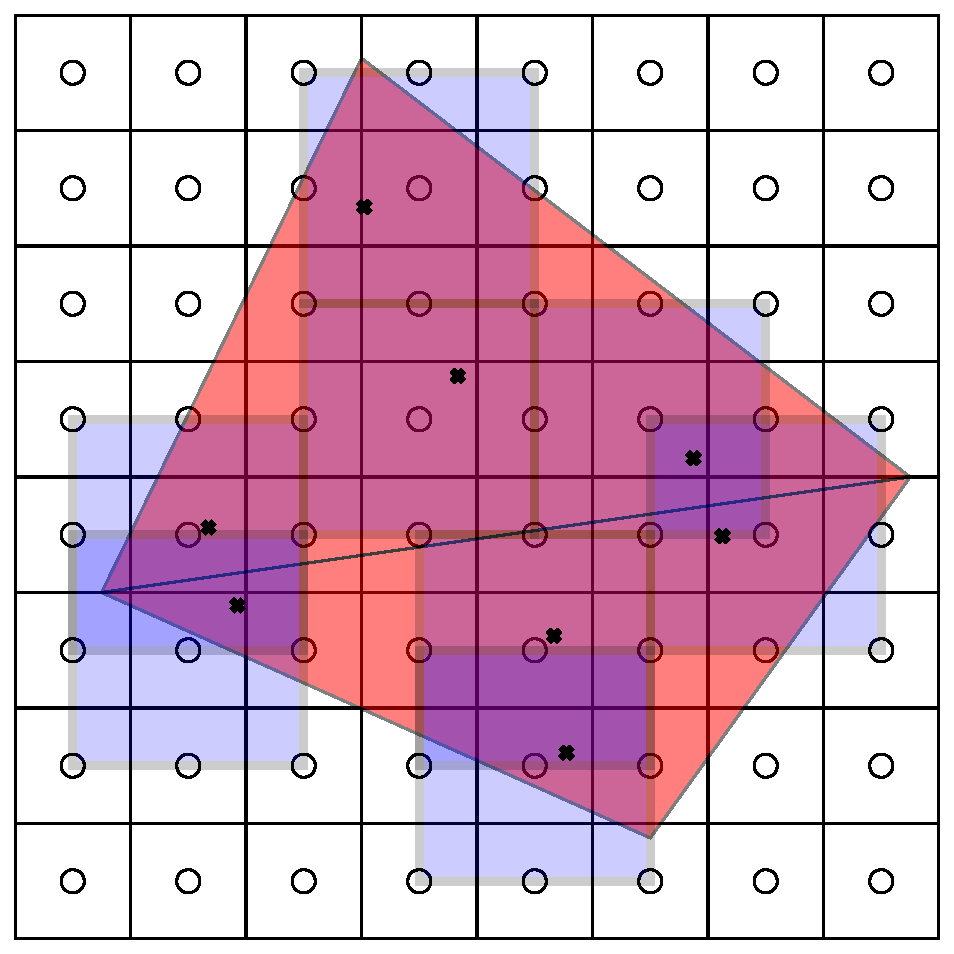
\includegraphics[width=0.4\linewidth]{interactionstencils/elemental_stencil.pdf} &
        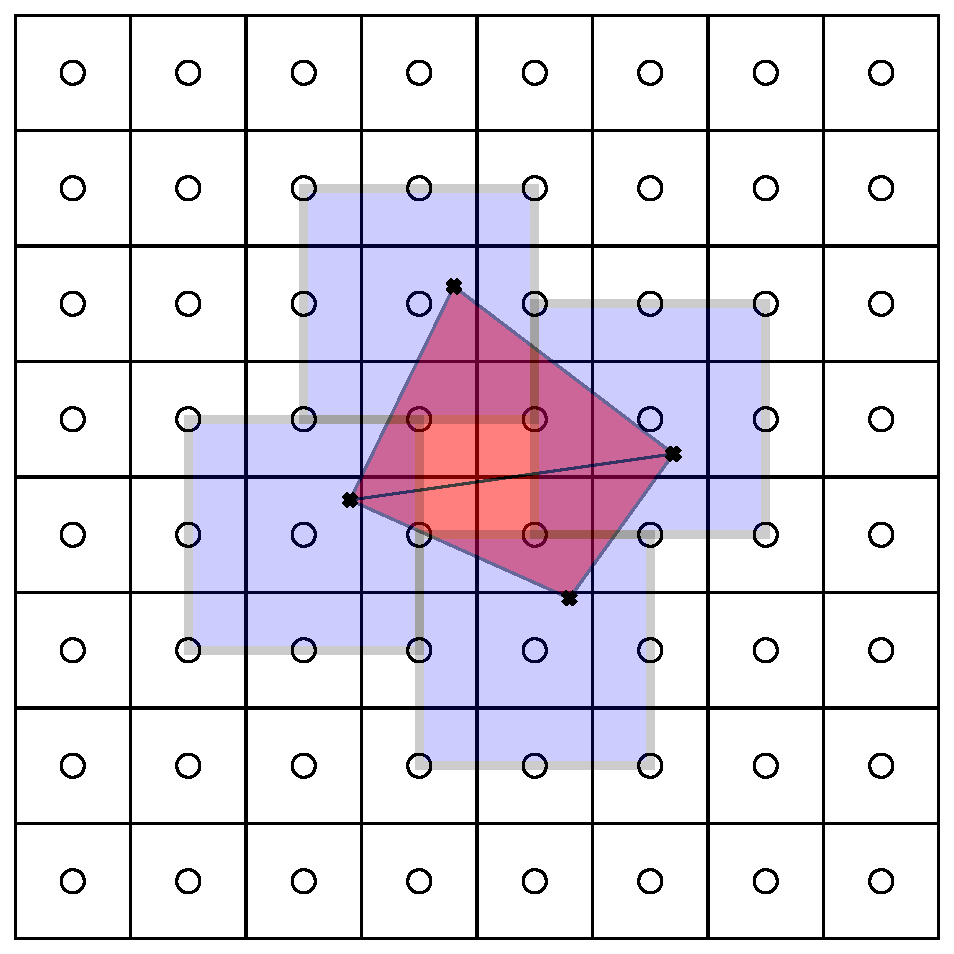
\includegraphics[width=0.4\linewidth]{interactionstencils/nodal_stencil.pdf}
      \end{tabular}

      Can either evaluate the integral operators with Gauss quadrature (left) or
      nodal quadrature (right). Not shown to scale!
    \end{figure}

    IBAMR implements FDM and IB methods - use deal.II for all unstructured grid things.
\end{frame}

\begin{frame}
    \frametitle{Explicit Mechanics} The implicit IB method is WIP for us. We
    do everything explicitly.

    \begin{itemize}
      \item Disadvantage of IB method: keeping structures in-place is hard
      \item Body forces (volumetric penalties, spring forces) (\texttt{cardinal::ForceContribution})
      \item Stresses (first Piola-Kirchoff: $\PPs(\Xb,t)$ from the equations
        slide) (also \texttt{cardinal::ForceContribution})
      \item Active strain models (don't use $\FF(\Xb,t)$ directly: `fix' it to
        only permit deformations in specified directions) (\texttt{cardinal::ActiveStrain})
    \end{itemize}

    \texttt{dealii::FEValues} is nice, we have \texttt{cardinal::MechanicsValues} to compute
    invariants, strains, etc. (and prevent users from calling \texttt{slowpow})
\end{frame}

\begin{frame}
    \frametitle{Goals}
    %%% TODO: picture!
    What is this project all about? Haven't people already done everything with the IB method?
    \begin{itemize}
      \item Immersed methods (not cut cells), neutral buoyancy. IFED now, IIM soon.
      \item Modern fiber-reinforced material models (e.g., Holzapfel-Gasser-Ogden).
      \item All features are available through input files.
      \item Parallel (FEBio has more features but will probably never support MPI).
      \item Students can do interesting things with it and \emph{not} write 5000 line monoliths
    \end{itemize}
\end{frame}

\begin{frame}
    \frametitle{Brief History of Cardinal}
    How did we get here?
    \begin{itemize}
      \item 2018: four-chambered-heart. Realistic valve dynamics with libMesh!
      \item 2020: deal.II with simplices is ``not impossible'' (what did we write on the wiki?)
      \item 2021: four-chambered-heart, IBAMR, deal.II (fiddle)
      \item 2022: I write another libMesh-based paper on nodal interaction
      \item 2023: Heart model (Davey) plus IFED (me) plus electrocardiology (Abdala, Rossi)
      \item 2024: Realistic valve dynamics with deal.II
    \end{itemize}
\end{frame}


\section{Rest of the talk}
\begin{frame}
  \frametitle{What is this talk about?}

  \begin{center}
    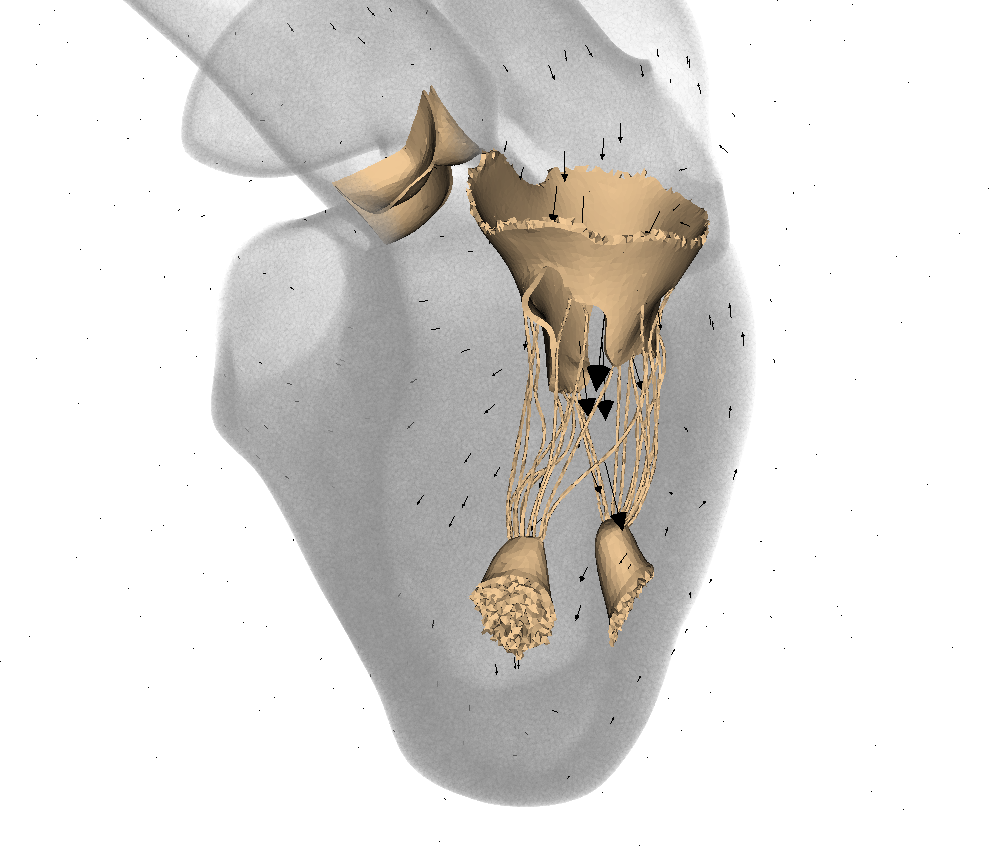
\includegraphics[width=0.4\linewidth]{mitral-2.png}
  \end{center}

  \begin{itemize}
    \item Problems Abdala and I ran into
    \item Interesting Cardinal features
    \item Ideas for improving other deal.II apps
  \end{itemize}

  \vfill

  \begin{center}
    Framing: eliminating the three kinds of waste (muri, muda, mura).
  \end{center}
\end{frame}

\section{Who are we?}
\begin{frame}
    \frametitle{Who are we?}
    We are...
    \begin{itemize}
      \item Faculty members, research scientists, postdocs
      \item Decades of C++ experience
      \item Formal training in mathematics, computer science
    \end{itemize}

    \vfill

    Our jobs are...
    \begin{itemize}
      \item dev ops (who is going to fix the CI?)
      \item write proposals
      \item teach classes
    \end{itemize}
    We can do anything, but we can't do everything.
\end{frame}

\begin{frame}
    \frametitle{Who are graduate students?}
    \begin{aquote}{W. Edwards Deming}
      Put a good person in a bad system and the bad system wins, no contest.
    \end{aquote}

    Students are...
    \begin{itemize}
      \item Smart
      \item Know a lot about subject areas (biomechanics, electrophysiology)
      \item New to scientific computing
    \end{itemize}

    \vfill
    Students do not have...
    \begin{itemize}
      \item Years of C++ experience
      \item Years of engineering experience
      \item Formal training in computer science
    \end{itemize}
\end{frame}

\section{Muri}
\begin{frame}
  \frametitle{Muri - Unreasonable, Over-burdening}
  Rule-of-thumb: students should succeed 85\% of the time, fail 15\% of the time

  Which tasks do students struggle with the most?
  \begin{itemize}
    \item C++
    \item Architecture (we should be the vanguard and rearguard)
    \item Installing things (students shouldn't spend days recompiling stuff)
  \end{itemize}
\end{frame}

\begin{frame}
  \frametitle{Muri - Unreasonable, Over-burdening}
  C++ is hard. How can we make it easier for students?
  \begin{itemize}
    \item \texttt{clang-format} (thanks Matthias!)
    \item Great documentation (deal.II's greatest strength)
    \item \texttt{-Wall -Wpedantic -Werror -DDEBUG} on the CI
    \item Constant-time accessors are named \texttt{get\_*()} (guaranteed to not
      use MPI, can be called in hot loops, etc)
    \item Most functions are named \texttt{compute\_*()}
    \item Don't worry about ADL et al: prefix member variables with \texttt{m\_}
    \item No Greek or shorthand, e.g., \texttt{bndry}
    \item I fight hard to keep CGS units everywhere
  \end{itemize}

  \vfill

  Abdala and I wrote the style guide together - we should keep students involved
  in writing standards!
\end{frame}

\begin{frame}
  \frametitle{Muri - Unreasonable, Over-burdening}
  C++ is hard. How can we make it easier for students?

  \begin{itemize}
    \item ``don't learn the tricks of the trade, learn the trade''
    \item ChatGPT frequently solves problems that don't need to be solved
    \item TODO: compile more good resources (keynotes, lecture series, books)
      for students to learn from instead of whatever ChatGPT recommends
  \end{itemize}
\end{frame}

\begin{frame}
  \frametitle{Muri - Unreasonable, Over-burdening}

  \begin{center}
    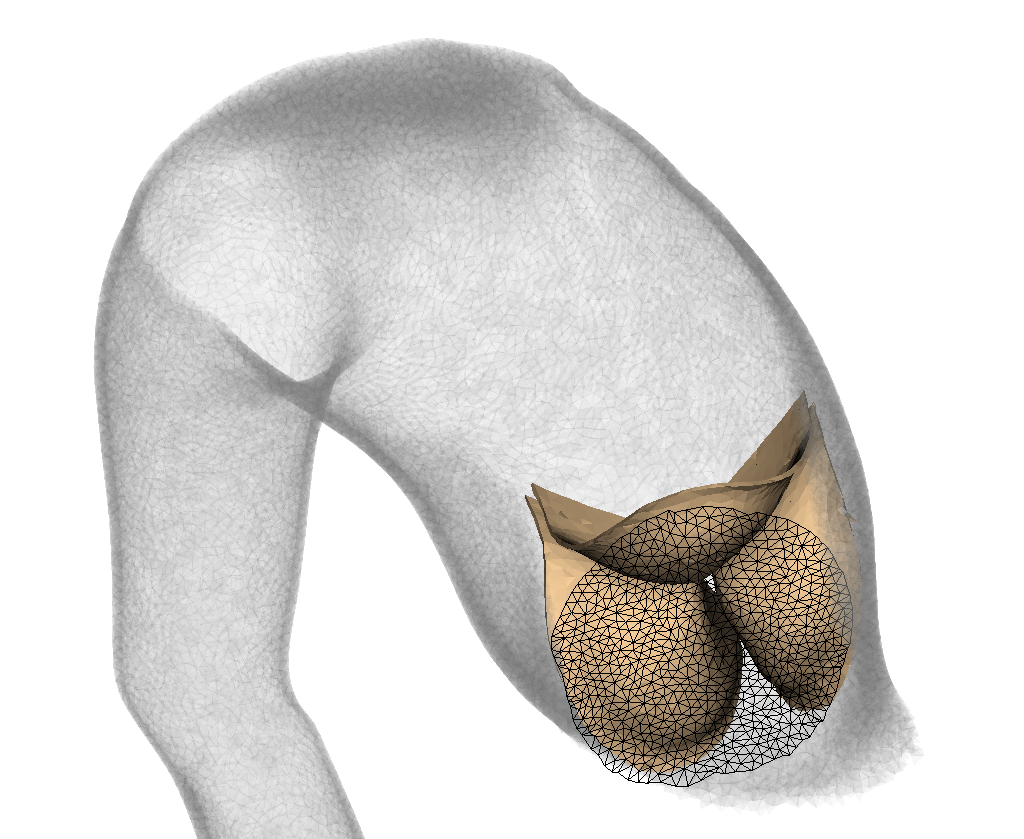
\includegraphics[width=0.4\linewidth]{tricuspid-1.png}
  \end{center}

  Provide good architecture so
  students don't have to solve every problem, just their problem.

  \begin{itemize}
    \item I spent a lot of time reading Aspect's source code (thanks!)
    \item Make it possible for students to get the job done by inheriting from a
      class, using a plugin, etc. instead of patching some huge class
  \end{itemize}
\end{frame}

\begin{frame}
  \frametitle{Overburdening: Use Good Architecture}

    How do we prevent students from writing 5000-line monoliths? How do we
    sustainably grow deal.II? What is deal.II?

    deal.II architecture:
    \begin{itemize}
      \item The very nice dependency graph on the front page of the manual
      \item \texttt{dealii::SmartPointer} and \texttt{dealii::Subscriptor}: one-to-many
      \item No global variables!
      \item All time-dependent state is in vectors, which are loosely coupled
        via \texttt{dealii::Utilities::MPI::Partitioner}
    \end{itemize}
\end{frame}

\begin{frame}
  \frametitle{Overburdening: Use Good Architecture}

    Cardinal architecture:
    \begin{itemize}
      \item `When in Rome': inherit several IBAMR-isms (SAMRAI's input files,
        restart singleton class)
      \item RAII, no staged initialization (not obvious to students!)
      \item Who is responsible? \texttt{std::move()} when we can,
        \texttt{subscribe()} if we must, \texttt{std::shared\_ptr} if absolutely
        necessary
      \item Like deal.II: most of the work happens in utility functions, classes
        (except FE vectors) are immutable modulo regridding
      \item Goal: everything accessible through the input file. Custom code via
        plugins
    \end{itemize}
\end{frame}

\begin{frame}
  \frametitle{Overburdening: Use Good Architecture}

    Cardinal architecture:
    \begin{itemize}
      \item Like Aspect: \texttt{main.cc} sets up the \texttt{cardinal::Simulator}
        God-object (unavoidable to write a reasonable time-stepping loop),
        catches exceptions
      \item Unlike Aspect: no \texttt{dlopen()} for plugins - they are
        explicitly passed to \texttt{cardinal::Simulator} (not sure which is better)
      \item Unlike Aspect: no \texttt{cardinal::SimulatorAccess} yet
    \end{itemize}
\end{frame}

\begin{frame}
  \frametitle{Overburdening: Use Good Architecture}

    Cardinal architecture: \texttt{cardinal::Part<dim, spacedim>}
    \begin{itemize}
      \item solely responsible for the position, velocity, and material models
        (forces, active strains) of one structure
      \item ctor: \texttt{std::vector<std::unique\_ptr<cardinal::ForceContribution<dim>>},
        \texttt{std::vector<std::unique\_ptr<cardinal::ActiveStrain<dim>>},
      \item uses RAII
      \item only place where we use \texttt{set\_*()} functions!
      \item \texttt{SmartPointer<const cardinal::Part<dim>>} grants access
    \end{itemize}
\end{frame}

\begin{frame}
  \frametitle{Overburdening: Use Good Architecture}

    Cardinal architecture: \texttt{cardinal::fsi::IFEDMethod<dim>}
    \begin{itemize}
      \item inherits from \texttt{IBAMR::IBStrategy}
      \item `handed-off' to \texttt{IBAMR::IBExplicitHierarchyIntegrator}
      \item ctor: \texttt{std::vector<cardinal::Part<dim>>} (unique ownership of
        \texttt{cardinal::Part}s)
      \item implementation: about 1500 LOC, all loops over cells are in utility functions
    \end{itemize}
\end{frame}

\begin{frame}
  \frametitle{Overburdening: simplify compilation}
  Students spend a \emph{shocking} amount of time recompiling stuff! Everything
  that can go wrong will frequently go wrong.

  \begin{itemize}
    \item Multiple copies of PETSc
    \item Conflicts between system libraries and user libraries
    \item Don't know what package managers are
  \end{itemize}

  Solution: autoibamr (forked from candi). Minimal configuration options
  (known-good versions, only three build types) means it is more likely to
  succeed. We should continue investing in anything that makes this process
  easier.
\end{frame}

\section{Muda}
\begin{frame}
  \frametitle{Muda - non-value-added work}
  \begin{aquote}{Sigeo Shingo}
    The most dangerous kind of waste is the waste we do not recognize.
  \end{aquote}
  What do we actually do that is of value?

  \vfill

  \begin{itemize}
    \item Graduate students
    \item Write papers
    \item Ship software
  \end{itemize}

  \vfill

  Everything else is either necessary (e.g., write grants) or unnecessary
  (should be removed).
\end{frame}

\begin{frame}
  \frametitle{non-value-added work: observations}

  What are our students actually doing?
  \begin{itemize}
    \item Compiling code (\emph{fixes}: ccache, CI, better hardware, use \texttt{-O1} or \texttt{-Os})
    \item Debugging (\emph{don't write bugs!})
    \item Running everything in debug mode (too slow!)
    \item Managing dependencies, upgrades, system administration
    \item Typing too slowly or inaccurately
  \end{itemize}
\end{frame}

\begin{frame}
  \frametitle{non-value-added work: compiling}

  Various performance improvements are not obvious - students don't have the vocabulary.
  \begin{itemize}
    \item \texttt{make} to \texttt{ninja} (what is \texttt{-j4}?)
    \item \texttt{-O3} to \texttt{-O1} (multiple builds?)
    \item \texttt{ccache} (what are object files?)
    \item Interesting linker developments (\texttt{ld}, \texttt{gold}, \texttt{mold})
    \item Make the CI fail fast
    \item Trickery to make \texttt{-DDEBUG} work with \texttt{-O1} in release mode
  \end{itemize}
\end{frame}

\begin{frame}
  \frametitle{non-value-added work: munging text files}

  \begin{center}
    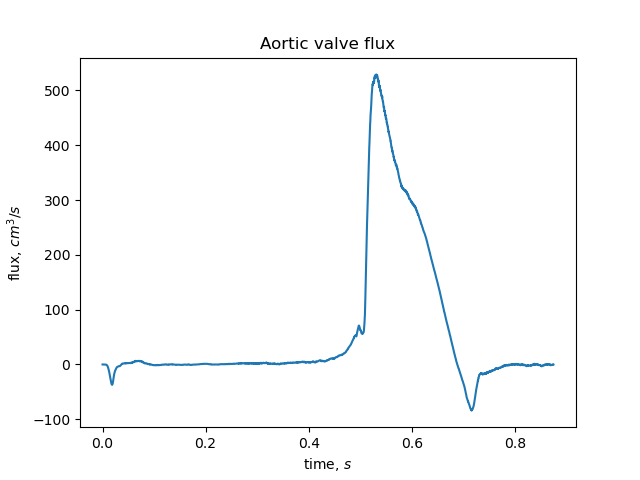
\includegraphics[width=0.6\linewidth]{aortic-valve-flux.png}
  \end{center}

  four-chambered-heart: Need to log something? Open a text file!
  \begin{itemize}
    \item Produces wrong output with restarts!
    \item What went where and why? How do we pick file names?
    \item Are we using mmHg today? Are you \emph{sure} it is mmHg?
  \end{itemize}
\end{frame}

\begin{frame}[fragile]
  \frametitle{non-value-added work: munging text files}

  We have a single class now for all output:
  \texttt{cardinal::StatisticalOutput}
  \begin{verbatim}
template <int dim>
struct Statistics
{
  std::string                                            group;
  std::map<std::string, std::pair<double, Unit>>         scalars;
  std::map<std::string, std::pair<Tensor<1, dim>, Unit>> vectors;
};
  \end{verbatim}

  \begin{itemize}
    \item Quite different from the Aspect version - uses 100\% HDF5 (structured
      output, stores units as metadata, etc), no \texttt{TableHandler}
    \item Works correctly with restart files
    \item IBAMR-ism: can load the HDF5 file as an input file
    \item Future work: callbacks, user-defined statistics via plugins
  \end{itemize}
\end{frame}

\section{Mura}
\begin{frame}
  \frametitle{Mura - patches, unevenness, non-uniformity}
  \begin{aquote}{Taiichi Ohno}
    Where there is no Standard there can be no Kaizen.
  \end{aquote}

  \vfill

  \begin{itemize}
    \item Georgetown's Camry plant: all jobs equally physically taxing, rotate to
      avoid RSI
    \item Bowling Green's Corvette plant: younger staff get harder jobs, more
      senior staff pick less taxing jobs
  \end{itemize}
\end{frame}

\begin{frame}
  \frametitle{Unevenness: definitions in scientific computing}

  What does this mean in scientific software?

  \vfill

  \begin{itemize}
    \item Try to level out the workload (e.g., having the CI automatically file issues)
    \item Minimize time between error creation and error detection
    \item Minimize time to merge new code
    \item Train students to break up work
    \item I refuse to review patches with more than 1k lines of source code changed
  \end{itemize}
\end{frame}

\begin{frame}[fragile]
  \frametitle{Unevenness: case example}

  \begin{verbatim}
for (unsigned int i = 0; m_ionic_parts.size(); i++)
    m_ionic_parts[i].save(archive, version);
  \end{verbatim}

  What went wrong here? Let's do 5-why!

  \vfill

  {\small
  \begin{verbatim}
An error occurred in line <1050> of file <[...]/source/base/utilities.cc>
 in function
 void [...]::posix_memalign([...])
The violated condition was:
 ierr == 0
Additional information:
 Your program tried to allocate some memory but this allocation failed.
 Typically, this either means that you simply do not have enough memory
 in your system, or that you are (erroneously) trying to allocate a
 chunk of memory that is simply beyond all reasonable size, for example
 because the size of the object has been computed incorrectly.

 In the current case, the request was for 18410715276690587648 bytes.
  \end{verbatim}
  }
\end{frame}

\begin{frame}
  \frametitle{Unevenness: case example}

  My program crashed in debug mode.
  \begin{enumerate}
    \item Why? My vector tries to allocate 16 exabytes of memory.
    \item Why? Clearly (to an expert) reading uninitialized memory.
    \item Why? Walked off the end of an array.
    \item Why? No range checks.
    \item Why? We don't have a way to turn on range checks automatically
  \end{enumerate}

  \vfill

  Now what?

  \begin{itemize}
    \item Starter fix: compile everything with
      \texttt{-D\_GLIBCXX\_ASSERTIONS} (easy)
    \item Better fix: set up CI to use \texttt{-D\_GLIBCXX\_DEBUG\_PEDANTIC},
      sanitizers (harder)
  \end{itemize}
\end{frame}


\end{document}
